\section{INTRODUCTION}

Consider a possible digital control system architecture
for use in a flight control system.  Sensors,  actuators, and
data networks are designed redundantly to mitigate faults.  In our 
proposed architecture the underlying platform 
implements a variant of the time-triggered architecture 
(TTA)~\cite{timed:tta}, which provides precise timing 
and reliability guarantees.  Safety-critical tasks 
and messages execute according to strict precomputed 
schedules to ensure synchronization between replicated 
components and provide fault mitigation and management.  
Deployed software implementations of the control functions must 
pass strict certification requirements which impose 
constraints on the software as well as on the development 
process.  The additional burden of design analysis required to 
establish safety increases cost and schedule, decreasing the
flexibility of the development process.

In modern embedded control system designs, graphical modeling
and simulation tools (e.g. Mathworks' Simulink/Stateflow) represent 
physical systems and engineering designs using block diagram notations. 
Design work revolves around simulation and test cases, with 
code generated from models when the design team reaches 
particular schedule milestones. Control designs often 
ignore software design constraints and issues arising 
from embedded platform choices. At early stages of the 
design, platforms may be vaguely specified to engineers 
as sets of trade offs~\cite{modeling:platform}.

Software development uses Unified Modeling Language 
Computer-Aided Software Engineering (UML CASE) tools to 
capture design artifacts and relationships such as types, components, 
interfaces, interactions,  timing, fault handling, and deployment.  Software development workflows focus on source code creation, organization, and management, followed by testing and debugging on target hardware. 
Physical and environmental constraints are often included in models, 
but the use of those constraints lies on the forefront of model-based
embedded systems research.  In many cases in practice such constraints 
only serve as documentation to developers and are encoded manually 
into test cases, losing many of the potential benefits of formally representing them in design models.

Complete control system software designs rely on multiple aspects.  
Designers lack tools to model the interactions 
between the hardware, software, and the environment 
with the required fidelity.  For example, software 
generated from a carefully simulated synchronous 
dataflow model of the controller functions 
may fail to perform correctly when 
its functions are distributed over a shared network of 
processing nodes.  Cost or availability considerations may force the
selection of platform hardware that limits timing accuracy 
or data precision beyond originally designed bounds.  
None of the current design, analysis,
or development techniques support comprehensive 
(i.e. multi-domain) validation of certification 
requirements to meet government safety standards. 
Model and code analysis tools must all be integrated to
have the same semantic view of the design details.

\subsection{Overview}

We aim to create a Domain Specific Modeling Language (DSML)
to address problems of design consistency across the entire 
development flow for a distributed embedded control system 
design.  Often, the best solutions involve iterating the 
design cycle as problems are discovered or problem understanding
increases.  Our DSML captures the relationships between 
concepts in the different design domains described, and supports
the integration of analysis tools and code generation.  The ultimate goal is to 
assess the performance and safety of code generated from the models in the context of the actual platform on which it will execute, subject to platform-induced delays and uncertainties.

\subsection*{High-Confidence Design Challenges}
\addcontentsline{toc}{subsection}{Design Challenges}

We identify several specific challenges that arise because of 
inconsistencies between domains in a high-confidence embedded 
development project.  Some of the challenges are fundamental,
and others arise because of our attempts to use models to
resolve consistency problems.

\begin{enumerate}
 \item Controller, software, and hardware design 
domains are highly specialized and often conceptually
incompatible.  Sharing model artifacts between 
designers in different domains can lead to consistency
problems in engineering solutions or implementations
based on incomplete or faulty understanding 
of design issues.  Current state of the art resolves 
differences in understanding by reviewing many of the details in 
numerous meetings and personal discussions.  
Manual reconciliation of issues occurs as individual
designers receive assignments to modify and correct 
the design. In the worst 
cases serious incompatibilities are not discovered 
until very late in the design cycle, leading to project 
overruns and cancellations\cite{prog:rapid_dev}.
Several large modeling tool projects 
(for example, AADL \cite{modeling:aadl_control_systems}
and Topcased\cite{tools:Topcased}) work to integrate tools 
from independent research and development teams into a 
common design environment featuring a standardized 
modeling language.  Resolution of semantic consistency
between integrated tools to improve design efficiency 
is a serious issue in such efforts.

 \item Incompatibilities between models and assumptions 
in different design domains create a related problem.  
For example, controller design properties which are verified 
using simulation models may no longer be valid
when the design becomes software in a distributed 
processing network.  Currently control designers 
use conservative performance margins to avoid rework 
when performance is lost due to deployment on a 
digital platform.

 \item Long development, deployment, and test cycles 
limit the amount of iterative rework that can be done
to get a correct design.  If a particular design analysis
is costly or time-consuming, the team cannot afford to 
iterate the design from its early stages in order to resolve
problems.  Currently high-confidence 
design requires both long schedules and high costs.

 \item Automating steps in different design and analysis 
domains for the same models and tools requires a consistent 
view of inferred model relationships across multiple design 
domains.  If integrated tools have different views of the 
model semantics, then their analyses are not valid when 
the results are integrated into the same design.
Therefore, all of the tools used in the design process must have a 
consistent view of design details.  Explicitly reconciling semantics 
between formalisms and tools is costly and time-consuming.  
Often the effort cannot be justified outside of academic 
research unless the results are applicable to numerous designs.

 \item As our research explores new directions in 
high-confidence design, modification of the ESMoL 
meta-model (language specification) creates maintenance 
problems for ESMoL models and for interpreter code 
that translates them into analysis artifacts and 
generated code.  We would like to isolate interpreter
development from the language to a degree in order 
to allow the ESMoL language to evolve with our research.  ESMoL models
can be updated to new versions of the language using 
features built into the tools, but nothing exists 
yet to handle those problems for interpreter code.  

\end{enumerate}

\subsection*{Model-Integrated Solutions}
\addcontentsline{toc}{subsection}{Solutions}
\label{section:solutions}

We propose a suite of tools
that aim to address many of these challenges.  Currently 
under development at Vanderbilt's Institute for Software 
Integrated Systems (ISIS), these tools use the Embedded 
Systems Modeling Language (ESMoL), which is a suite of 
domain-specific modeling languages (DSML) to integrate the 
disparate aspects of a safety-critical embedded systems design 
and maintain proper separation of concerns between control 
engineering, hardware specification, and software development 
teams.  The Embedded Systems Modeling Language (ESMoL) encodes 
in models the relationships between controller functions
specified in Simulink, software components that implement
those functions (i.e. dataflow, messaging interfaces, 
etc\ldots), and the hardware platform on which the software
will run.  Many of the concepts and features presented here also 
exist separately in other tools.  We describe a model-based 
approach to building a unified model-based design and 
integration tool suite which has the potential to go far 
beyond the state of the art.

\begin{enumerate}
 \item The ESMoL language and tools provide a single 
multi-aspect embedded software design environment 
so that modeling, analysis, 
simulation, and code generation artifacts are all 
clearly related to a single design model.  We aim to incorporate
models appropriate to the different design domains 
in a consistent way using the Model-Integrated Computing (MIC)
approach discussed below.
ESMoL models use language-specified relations to associate Simulink 
control design structures with
software and hardware design concepts to define a
software implementation for controllers.
Further, ESMoL is a graphical modeling language which integrates 
into existing Simulink-based control design work flows\cite{modeling:esmol}. 

 \item ESMoL models include objects and parameters 
to describe deployment of software components to 
hardware platforms.  Analysis artifacts and simulation 
models generated from ESMoL models contain 
representations of the behavioral effects of the 
platform on the original design.
We include platform-specific simulations to 
assess the effects of distributed computation on
the control design \cite{modeling:truetime}.

 \item ESMoL's integrated analysis, simulation, 
and deployment capabilities can shorten design cycles.
The ESMoL tool suite includes integrated scheduling analysis
tools(\cite{sched:analysis})
so that static schedules can be calculated in rapid design and
simulation cycles.  We include automatic generation of platform-specific
task configuration and data communications code in order to
rapidly move from modeling and analysis to testing on actual hardware.

 \item ESMoL uses a two-stage interpreter architecture 
in order to integrate analysis tools and code
generators.  The first stage resolves any inferred model 
relationships from ESMoL models into a model in 
an abstract language (ESMoL\_Abstract), much in the same 
way that a parser creates an abstract syntax tree 
for a program under compilation.  The ESMoL design language
allows relational inference where appropriate in order 
to make the designer more productive.  The Stage 1 
interpreter resolves object instances, parameters, and 
relations, and stores them in an ESMoL\_Abstract model.  
Model interpreters for analysis and generation use this 
expanded model to guarantee a consistent view of the 
relationships and details, and to share code efficiently 
in an integrated modeling tool development project.  The 
two-stage approach also isolates the interpreter code from 
the structure of the ESMoL language.  Changes to the 
language are principally isolated from the interpreter
code by the first stage transformation.

\item We generate analysis models and code from the intermediate language
using simple template generation techniques\cite{sched:analysis}.
Round-trip incorporation of calculated schedule 
analysis results back into the ESMoL model helps to
maintain consistency as models pass between design phases.

\end{enumerate}

\begin{figure}
\centering
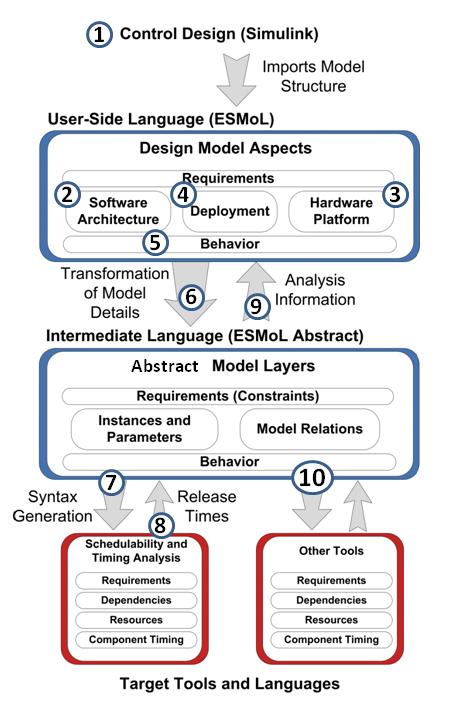
\includegraphics[width=0.7\columnwidth]{figures/designflow.png}
    \caption{Flow of ESMoL design models between design phases. }
    \label{fig:designflow}
\end{figure}

Fig. \ref{fig:designflow} depicts a design flow that 
includes a user-facing modeling language 
for design and an abstract intermediate language for 
supporting interpreter development and
maintenance.  During design, a software modeler imports 
an existing Simulink control design into 
the Generic Modeling Environment (GME) \cite{mic:gme}, 
configured to edit ESMoL models (Step 1).  The modeler
then uses the dataflow models imported from Simulink
to specify the functions of software components
which will be used to implement the controllers.  These component
specifications represent the behavior of synchronously executing C code compiled from a dataflow model,  and which are extended with interfaces defining 
input and output message structures for data distribution. 
We also specify the mapping from dataflow I/O ports to and from fields 
in the messages (Step 2).  
Designers specify the hardware topology for a time-triggered 
distributed processing network using another integrated 
design language (Step 3).
A modeler instantiates component instances to create multi-aspect 
models where logical dependencies, hardware deployment, and timing 
models can be specified for the software architecture (Steps 4 and 5).
Note that the requirements called out in the diagram are still conceptual.  We have language elements for capturing end-to-end latency specifications, but more general formal requirements capture is a possible future effort for ESMoL.

A completed model is transformed (via the Stage 1 
transformation) into a model in the ESMoL\_Abstract 
language, resolving all implied relationships and structural 
model inferences (Step 6).  Model interpreters 
for design analysis (in this case calculating time-triggered 
schedules) are integrated using the Stage 2 model 
transformation from ESMoL\_Abstract models to analysis
specifications (Step 7).  Another model interpreter imports 
results from the analysis (in this case, scheduled start times) 
back into the ESMoL\_Abstract and ESMoL models (Steps 8 and 9).
Finally, designers can also create 
platform-specific simulations and generate deployable 
code using the Stage 2 transformation (Step 10).

In a later section we discuss the relationship between the behavior represented
by the original Simulink model and the behaviors represented by ESMoL and
ESMoL\_Abstract (Steps 5 and 10).  ESMoL provides a great deal of modeling
flexibility, as subsets of the Simulink model are used in Step 2 to 
define software components.  These subsets can be replicated to model 
redundant computation networks, for example.  In Step 4 they are aggregated to 
define dataflows, and then partitioned to define deployment of those dataflows.
With all of the language flexibility provided, we need to ensure that the 
synchronous semantics of the original Simulink model are preserved in
the distributed implementation in order to
ensure that the inherent correctness properties (functional determinism,
timing determinacy, and deadlock freedom) are also preserved.

The illustrated design flow represents only a single iteration in 
the overall development work flow to be discussed later.  
In the sequel we will use the 
expression \emph{design flow} to indicate the work of modeling,
analyzing, and generating code for a single design.  \emph{Development flow}
will indicate the macro-level iterative development process
which includes one or more design flow iterations.

